
\section{Graphs}

A graph is a pair $G = (V,E)$ where $V$ is a finite set, and $E$ is a set of
pairs between items in $V$. Elements in $V$ are \textit{vertices} or
\textit{nodes}, and elements in $E$ are \textit{edges}.

Different mathematicians have different rules about what exactly can go in a
graph. For the purposes of this course, the graphs shown in
Figure~\ref{fig:bad-graphs} aren't allowed.

\begin{figure}[h]
  \centering
  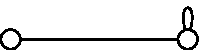
\includegraphics{diagrams/self-loops}\\
  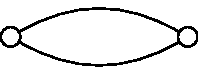
\includegraphics{diagrams/multiple-edges}\\
  
\includegraphics{diagrams/directed-graph}
  \caption{Self loops, duplicate edges and arrows are not allowed.}
  \label{fig:bad-graphs}
\end{figure}

A \textbf{directed graph} is just like a normal graph, except the edges do have
arrows. The only mathematical difference is that the set $E$ is a set of ordered
pairs. The third diagram in Figure~\ref{fig:bad-graphs} is a directed graph (it
is always referred to as a directed graph!).

The \textit{degree} of a node in a graph, is the number of edges that are
adjacent to (touching) it. If the graph is directed, then it is the number of
edges originating from the node.

A weighted graph is one where each edge is associated with a value representing
its weight. The length of a path between nodes is simply the sum of the edge
weights connecting the nodes.

\subsection{Connectivity}
\label{connectivity}

A node $a$ is \textbf{reachable} from another node $b$ if there is some sequence
of nodes connected by edges that go from the $a$ to $b$.

A graph where every node is reachable from every other node is
\textbf{connected}. A strongly connected graph is a \textbf{directed graph}
where each node is reachable from each other node.

\begin{figure}[h]
  \centering
  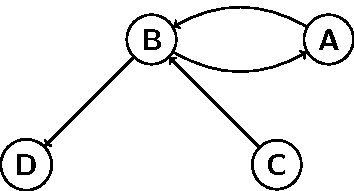
\includegraphics{diagrams/connected-graph}
  \caption{This graph is not strongly connected, but the subgraph with only
  nodes $A$ and $B$ is. If we were to remove the arrows, then the graph would
  be connected.}
  \label{fig:connected-graph}
\end{figure}

\subsection{Representing graphs}

We can store graphs in computer memory in two ways:

\begin{description}
  \item \textbf{Adjacency List}\\
    There are two different kinds of adjacency list, the first is like so:

    \begin{lstlisting}[language=java]
      public class Graph {
        List<Vertex> nodes;
        List<Edge> edges;
      }
      public class Edge { Vertex a, b; }
      public class Vertex { List<Edge> outlist; }
    \end{lstlisting}

    Here, we keep a list of all the nodes, and a list of all the edges. From
    any edge, we can see what nodes it connects, and from any node, we can
    see what edges it connects.

    The other type of adjacency list is a bit simpler, but less efficient in
    some cases:

    \begin{lstlisting}[language=java]
      public class Graph<T> {
        Set<T, List<T>> adjList;
      }
    \end{lstlisting}
  \item \textbf{Adjacency Matrix}\\
    Here, a matrix indicates whether there is an edge between two nodes:

    \begin{center}
      \begin{tabular}{c|c c c c}
          & A & B & C & D\\ \hline
        A & 0 & 1 & 0 & 0\\
        B & 1 & 0 & 0 & 1\\
        C & 0 & 1 & 0 & 0\\
        D & 0 & 0 & 0 & 0\\
      \end{tabular}
    \end{center}

    This adjacency matrix represents the graph in
    Figure~\ref{fig:connected-graph}. You can see that it is fairly wasteful
    in terms of memory $O(|E|* |V|)$, though with bit arrays, it has a very 
    low constant overhead.
\end{description}

\subsection{Classifying Edges}

During a \textit{depth first traversal} (Section~\ref{depth-first-search}) of a
graph, we can classify each edge into one of four types. When doing the
traversal, we process each edge from left to right (from the viewer's
perspective), and we define an edge to be an \textit{ancestor} of another edge
if there is a path from the ancestor edge to the descendent edge and the ancestor
is traversed first. The four types of edges are:

\begin{description}
  \item \textbf{Tree edges}\\
    These edges lead to a new node during a search. If you remove all the edges 
    from the graph except tree edges, then you get a tree!
  \item \textbf{Forward edges}\\
    These go from ancestor edges to descendent edges, but are not tree edges
    (i.e. the descendent node has been visited already).
  \item \textbf{Cross edges}\\
    These go between edges where no node is the ancestor of the other.
  \item \textbf{Back edges}\\
    An edge that goes from a descendant to an ancestor.
\end{description}

\begin{figure}[h]
  \centering
  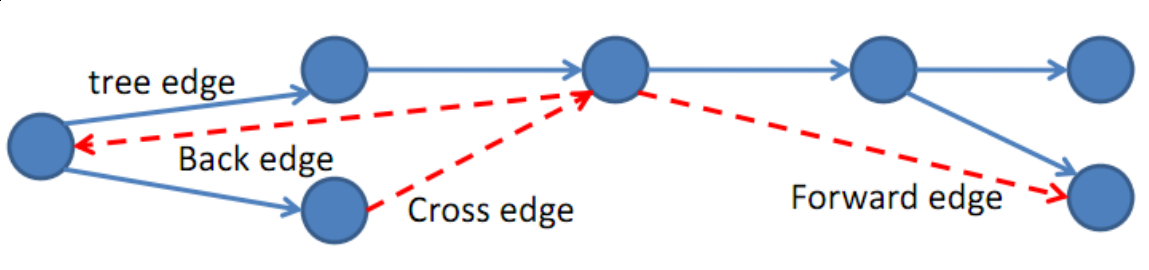
\includegraphics[width=0.6\textwidth]{images/edge-types}
  \caption{A
  \href{http://courses.csail.mit.edu/6.006/spring11/rec/rec13.pdf}{pictorial
  illustration} of the different edge types.}
  \label{fig:connected-graph-edge}
\end{figure}

\subsection{Graph Algorithms}

You will have covered some of the algorithms featuring here in previous courses,
or perhaps seen them in the wild. They are however interesting and useful, so
it's worth a recap even if they're not new! I've ordered these in roughly
increasing order of mental strain.

\subsubsection{Depth first search}
\label{depth-first-search}

\href{https://en.wikipedia.org/wiki/Depth-first_search}{Depth first search}
(DFS) is an algorithm to find a node in a graph starting from another node. It
works on both directed and undirected graphs, and runs in $O(|V| + |E|)$
(linear) time. The psudo code looks like this:

\marginpar{Note how we mark nodes as having been visited (by adding them to
\texttt{visitedNodes}). This is so if there is a loop in the graph, the 
algorithm doesn't run indefinitely.}

\begin{lstlisting}[language=java]
  Node dfs(Node haystack, Node needle) {
    Stack<Node> toVisit = new Stack<>();
    Set<Node> visitedNodes = new Set<>();
    toVisit.push(haystack);
    while(!toVisit.isEmpty()) {
      Node node = toVisit.pop();
      if (visitedNodes.contains(node)) continue;
      visitedNodes.add(node);
      if(node.equals(needle)) {
        return needle;
      } else {
        for(Node child : node.children) {
          toVisit.push(child);
        }
      }
    }
    return null;
  }
\end{lstlisting}

A Breadth First Search is the same, except you use a \texttt{Queue} instead of a
\texttt{Stack}.

\marginpar{To see if a graph is connected, do a depth first search as in the
example code, but don't stop when you find a needle, only stop when the
\texttt{toVisit} stack is empty. If \texttt{visitedNodes} contains all of the
nodes in the graph, then the graph is connected.}

Depth first search also lets you find if one node is reachable from another in
linear time, and also if a graph is connected in linear time too, with a few
modifications.

We can also find out if a directed graph is strongly connected in $O(|V| + |E|)$
time using Tarjan's algorithm, which we'll see later.

\subsubsection{Dijkstra's algorithm}

Dijkstra's algorithm finds the undirected shortest path between two nodes in a
graph. Here is the psudo-code:

\marginpar{My best advice for learning an algorithm like this, is to get a 
whiteboard, draw out the problem, and then run the solution manually on the 
whiteboard. Then you have a pictorial and visual explanation of how the 
algorithm \textit{really} works.}

\begin{lstlisting}[language=java,
                  caption=Dijkstra's algorithm (from Wikipedia),
                  label=lst:dijkstra,
                  captionpos=b]
function Dijkstra(Graph, source):
  create vertex set Q

  // Initialization
  for each vertex v in Graph:
    dist[v] = INFINITY
    prev[v] = UNDEFINED
    add v to Q

  // Distance from source to source
  dist[source] = 0

  while Q is not empty:
    u = vertex in Q with min dist[u]
    remove u from Q 

  for each neighbour v of u:
    alt = dist[u] + length(u, v)
    // A shorter path to v has been found
    if alt < dist[v]:
      dist[v] = alt 
      prev[v] = u 

  return dist[], prev[]
\end{lstlisting}

\marginpar{Remember, the maximum value of $E$ is actually $V^2$, and you can
sometimes use that to play with the runtime bounds of graph algorithms (e.g. you
could show something is linear in the number of edges, or polynomial in the
number of nodes).}

If we use a Fibonacci heap, for the priority queue, then the runtime of
Dijkstra's algorithm is $O(|E| + |V|log(|V|)$. If we use a normal heap, then the
runtime is $O((|E|+|V|)log(|V|))$.

\subsubsection{Tarjan's Algorithm}

Before we delve into Tarjan's Algorithm, we need to discuss strongly connected
components. You will remember from Section~\ref{connectivity}, that a graph is
strongly connected if all nodes are reachable from any other node.

A \textit{strongly connected component} is a subset of edges within a graph,
where the subset is strongly connected. If a graph has only one strongly
connected component, then it is strongly connected.

The psudo code here is from
\href{https://en.wikipedia.org/wiki/Tarjan%27s_strongly_connected_components_algorithm}{Wikipedia}.
If you're reading this after week 8 of the \texttt{COMP36111} course, then you
probably have your own implementation in C.

\begin{lstlisting}
  algorithm tarjan is
  input: graph G = (V, E)
  output: set of strongly connected components (sets of vertices)

  index := 0
  S := empty
  for each v in V do
    if (v.index is undefined) then
      strongconnect(v)
    end if
  end for

  function strongconnect(v)
    // Set the depth index for v to the smallest unused index
    v.index := index
    v.lowlink := index
    index := index + 1
    S.push(v)
    v.onStack := true

    // Consider successors of v
    for each (v, w) in E do
      if (w.index is undefined) then
        // Successor w has not yet been visited; recurse on it
        strongconnect(w)
        v.lowlink  := min(v.lowlink, w.lowlink)
      else if (w.onStack) then
        // Successor w is in stack S and hence in the current SCC
        v.lowlink  := min(v.lowlink, w.index)
      end if
    end for

    // If v is a root node, pop the stack and generate an SCC
    if (v.lowlink = v.index) then
      start a new strongly connected component
      repeat
        w := S.pop()
        w.onStack := false
        add w to current strongly connected component
      while (w != v)
      output the current strongly connected component
    end if
  end function
\end{lstlisting}

The algorithm basically applies a depth first search to the graph, and keeps
track of two properties (the index and the lowlink) for each node. The index is
the logical time at which the node was discovered by the algorithm, and the
lowlink is the index of the oldest ancestor that can be reached from the current
node.

Once the index has been assigned, it never changes. However, the lowlink is
updated during recursive depth first search calls to find back edges between the
node and its ancestors.

If any node has its index as the same value as its lowlink, then it is the root
of a strongly connected component (possibly only containing itself). Nodes will
be popped off the stack until the current node is removed, at which point we
have found all the nodes in this component.

If all nodes have not been discovered after a single depth first search, the
algorithm is run again on a previously undiscovered node. This ensures that all
the strongly connected components are found, even in graphs that have completely
disjoint components.

\subsubsection{Graph Colouring}

Graph colouring is a problem where we want to assign colours to nodes in a
graph, but no adjacent node can have the same colour. A \textit{k-colouring} of
a graph $G$ is a function $f : V \rightarrow \{ 0, 1, \dots, k - 1 \}$ such that
for any edge $(u, v) \in E, f(u) \neq f(v)$, and the output from $f$ is each
node's colour.

For some graphs, there is no valid colouring with $k$ colours. A graph is
\textit{k-colourable} if there exists a \textit{k-colouring} for that graph.

Of course, we can write a Turing Machine that can solve
\textit{k-colourability}. We can encode a graph by writing $n$ as the number of
nodes, and the pairs as the edges between them:

\[
  (n, (u_1, v_1), \dots, (u_m, v_m))
\]

See Section~\ref{sat-colour} for more on this!

\subsubsection{Hamiltonian Circuits}

{\tiny \vspace{-2em} You might want to read the later sections about complexity 
theory before this bit.}

A circuit of a graph is a path through the graph where every node is visited at
least once. An Eulerian circuit of a graph is where each edge is traversed
\textit{exactly} once, and a Hamiltonian circuit is one where each node is
visited exactly once.

\marginpar{Finding if a graph has a Eulerian Circuit is solvable in
\texttt{PTime}, since we simply have to check if every node has an even
out-degree, which can be done in $O(n^2)$.}

We're going to show that finding a Hamiltonian Circuit is a problem in
\texttt{NPTime}. We can do this in one of two ways; either to give a
nondeterministic Turing machine that will find a path in polynomial time, or we
can come up with a deterministic polynomial time algorithm to verify that a
given path is Hamiltonian.

You might be thinking \textit{``ummm, how can simply giving a polynomial time
verification algorithm show that we're in \texttt{NPTime}?''}; that's what I
thought at first. However, we could simply try all combinations of input to the
verifier and see if there is one that is Hamiltonian. This would work in
deterministic \texttt{ExpTime}, which can be computed in \texttt{NPTime}.

In order to show that trying to find a Hamiltonian path in a graph is
\texttt{NPTime-Complete}, we must map it to another \texttt{NPTime-Complete} 
problem. The course notes (lecture 9) does this by mapping it to \texttt{3-SAT} 
like we do for graph colouring in Section~\ref{sat-colour}.

We can use the fact that finding Hamiltonian Circuits is
\texttt{NPTime-Complete} to show that the Travelling Salesman problem is
\texttt{NP-Hard}, and then \texttt{NP-Complete}.

\marginpar{I've not shown how I computed the path with the matrix, but I did it 
on a whiteboard by crossing out used paths on the matrix. Giving a full 
explanation here would take too long now, and its not strictly on the syllabus.}

To do this, we construct a $N \times N$ matrix, where $1$ corresponds to an edge
between nodes and $2$ is for no edge. If we had a graph like in
Figure~\ref{tsp:graph}, then we could produce a matrix like in
Table~\ref{tsp:matrix}.

\begin{figure}[h]
\centering
\begin{subfigure}{.5\textwidth}
  \centering
  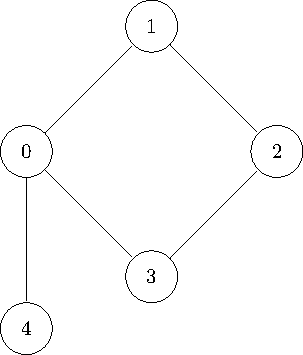
\includegraphics[width=.4\linewidth]{diagrams/graph15}
  \caption{The input graph}
  \label{tsp:graph}
\end{subfigure}%
\begin{subfigure}{.5\textwidth}
  \begin{tabularx}{0.2\textwidth}{M|M|M|M|M|MX}
      & 0 & 1 & 2 & 3 & 4\\ \cline{1-6}
    0 & 2 & 1 & 2 & 1 & \tikzmark{a}{1}\\
    1 & \tikzmark{b}{1} & 2 & 1 & 2 & 2\\
    2 & 2 & \tikzmark{c}{1} & 2 & 1 & 2\\
    3 & 1 & 2 & \tikzmark{d}{1} & 2 & 2\\
    4 & \tikzmark{e}{1} & 2 & 2 & 2 & 2
  \end{tabularx}
  \link{b}{a}
  \link{c}{b}
  \link{d}{c}
  \link{a}{e}
  \caption{The resulting matrix; start at 3, move to 2, then 1, then 0 and
  finally 4.}
  \label{tsp:matrix}
\end{subfigure}
\caption{Transforming the Hamiltonian Cycle problem to the TSP problem.}
\end{figure}

If the TSP problem finds a path with a total cost of less than or equal to $n$,
then there will be a Hamiltonian path, like in the figure. This means that TSP
is \texttt{NP-hard}. To show that it is \texttt{NP-Complete}, observe that TSP
is in \texttt{NP}, which is easy, since we can obviously verify that a given
path can be taken with a specific cost in polynomial time.
